% A good introduction to latex can be found here:
%  http://www.cse.ohio-state.edu/~hank/latex/lshort141.pdf

\documentclass{article}
\usepackage{amsmath}

\usepackage{full page}  % make the margins somewhat smaller than the default

\usepackage{listings}  %  needed for source code listings
\usepackage{color}
\usepackage{hyperref}
\usepackage{graphicx}
\usepackage[tight,footnotesize]{subfigure}

\definecolor{javared}{rgb}{0.7,0,0} % for strings
\definecolor{javagreen}{rgb}{0.25,0.6,0.35} % comments
\definecolor{javapurple}{rgb}{0.55,0,0.40} % keywords
\definecolor{javadocblue}{rgb}{0.25,0.35,0.85} % javadoc

\definecolor{pblue}{rgb}{0.13,0.13,1}
\definecolor{pgreen}{rgb}{0,0.5,0}
\definecolor{pred}{rgb}{0.9,0,0}
\definecolor{pgrey}{rgb}{0.46,0.45,0.48}
 
\lstset{language=Java,
basicstyle=\ttfamily,
  commentstyle=\color{pgreen},
  keywordstyle=\color{pblue},
  stringstyle=\color{pred},
morecomment=[s][\color{javadocblue}]{/**}{*/},
numbers=left,
numberstyle=\tiny\color{black},
stepnumber=2,
numbersep=10pt,
tabsize=4,
showspaces=false,
showstringspaces=false,
frame=shadowbox,
numbers=left,
%escapechar=\@
} 

% set the document title, author, and date here.
%  once set, the \maketitle command (within the document)
%  will display them nicely
\title{Chess AI}
\author{Junjie Guan $<gjj@cs.dartmouth.edu>$}

\begin{document}
\maketitle

\tableofcontents

\section{Introduction}

Adversarial search is an import area of AI, which can be applied to many real world games. One representation is Chess game.  In this report I am going build a chess AI and enhance it step by step. Section 2 to 8 will most talk about the ideas and implementations, including Minimax, Alpha-beta pruning, transposition table, moves reodering, null move heuristic, quiescence search, and finally a contorller to better operate the game. Section 9 will mostly contain the analysis and comparison of those AIs. Section 10 talk about some reading materials. 













\clearpage
\section{Minimax Search}
\subsection{Basic Idea}
In the realworld games, when making strategy, we not only try to make the best move for current situation, but also need to predict the reaction of adversary. Human brains are usually good at sniffing the useful information, but weak at processing too much information. While computer can process much more information than normal peole, it usually try to enumerate all the possible situation regardless of whether it is informative.

The first algorithm that I am going to introduce is minimax search. Though it has low efficiency, it is  the base of all other algorithms that I am going to introduce. The basic idea is to enumerate all the possible moves of the whole game. When we finish enuerating one players and then expand the moves of others based on the current expanded moves, we call it one depth deeper. The number of moves grows exponentially with depth. The structure is like a k-ary tree.

\subsection{Code implementation}


\subsubsection{minimaxIDS}

\textbf{minimaxIDS} initializes the search using iterative-depending strategy.


\begin{lstlisting}[numbers=left]
private short minimaxIDS(Position position, int maxDepth) 
    throws IllegalMoveException{
  this.terminalFound = false;
  MoveValuePair bestMove = new MoveValuePair();
  for (int d = 1; d <= maxDepth && !this.terminalFound; d++) {
    bestMove = maxMinValue(position, maxDepth - 1, MAX_TURN);
  }
  return bestMove.move;
}
\end{lstlisting}


\subsubsection{maxMinValue}

\textbf{maxMinValue} is an recursive funciton that keep searching in the tree. I write it in a compact way by mering min and max procedure in this one method, which turns out to be a big mistake for future when I try to implement more fancy mechansim for the searching. This design makes the codes a little messy.

There is also another better way to implement the search in a compact way, which is called \emph{Nagamax}. However it was too late for me to discover it so I leave it to my future work.

\begin{lstlisting}[numbers=left]
private MoveValuePair maxMinValue(Position position, int depth, 
    boolean maxTurn) throws IllegalMoveException{
  if (depth <= 0 || position.isTerminal()) {
    // the base case of recursion
    return handleTerminal(position, maxTurn);
  } else {
    // get all the legal moves
    MoveValuePair bestMove = new MoveValuePair();
    for (short move : position.getAllMoves()) {
      // collect values from further moves by recursion
      position.doMove(move);
      MoveValuePair childMove = maxMinValue(position, depth - 1, !maxTurn);
      bestMove.updateMinMax(move, childMove.eval, maxTurn);
      position.undoMove();
    }
    return bestMove;
  }
}
\end{lstlisting}

\subsubsection{handleTerminal}

\textbf{handleTerminal} is used to terminate the searching by returning an evalution value, when either reaching the maximun depth or check mate or draw. Noted that getMaterial evalutes the weighted sum of the stones, while getDominant evaluates the distribution of the stones.

\begin{lstlisting}[numbers=left]
private MoveValuePair handleTerminal(Position position, boolean maxTurn) {
  MoveValuePair finalMove = new MoveValuePair();
  if (position.isTerminal() && position.isMate()) {
    this.terminalFound = position.isTerminal();
    finalMove.eval = (maxTurn ? BE_MATED : MATE);
  } else if (position.isTerminal() && position.isStaleMate())
     finalMove.eval = 0;
  else {
    finalMove.eval = (int) ( (maxTurn ? 1 : -1) * (position.getMaterial() 
       + position.getDomination()));
  }
  return finalMove;
}
\end{lstlisting}

\subsubsection{helper class}

\textbf{MoveValuePair} help me to store the move and corresponding evaluation value. Also it has a generalized method that help me to find the max value for maximum search, or vise versa.

\begin{lstlisting}[numbers=left]
private MoveValuePair handleTerminal(Position position, boolean maxTurn) {
  MoveValuePair finalMove = new MoveValuePair();
  if (position.isTerminal() && position.isMate()) {
    this.terminalFound = position.isTerminal();
    finalMove.eval = (maxTurn ? BE_MATED : MATE);
  } else if (position.isTerminal() && position.isStaleMate())
     finalMove.eval = 0;
  else {
    finalMove.eval = (maxTurn ? 1 : -1) * position.getMaterial();
  }
  return finalMove;
}
\end{lstlisting}















\clearpage
\section{Alpha-beta pruning}
\subsection{Basic Idea}
The basic idea of RRT is to cutoff the those subtrees that do not affect the our final decision. For example, a parent tries to find the maximun decision provided by its children. So if your siblings already provider a decision that is already higher than your current upper bound or smaller than your lower bound, your decision will definitely be ignored, so there is no point to continue searching.

\subsection{Code implementation}

I extend the ABPrunign class from the previous Minimax class, so that we can reuse most of the function such as \textbf{maxMinValue}, \textbf{handleTerminal} and the helper class.

\subsubsection{ABMaxMinValue}

\textbf{ABMaxMinValue} is pretty much the same as the previous MinimaxValue method, with additional codes from line 15-20. You can see that the code is already a little clumsy and hard to read. (Though \emph{Nagamax} is also not that straight forward)

\begin{lstlisting}[numbers=left]
protected MoveValuePair ABMaxMinValue(Position position, int depth,
   int alpha, int beta, boolean maxTurn) throws IllegalMoveException {
  if (depth <= 0 || position.isTerminal()) {
    return handleTerminal(position, maxTurn);
  } else {
    MoveValuePair bestMove = new MoveValuePair();
    for (short move : position.getAllMoves()) {
      // collect values from further moves
      position.doMove(move);
      MoveValuePair childMove = ABMaxMinValue(position, depth - 1, alpha,
        beta, !maxTurn);
      bestMove.updateMinMax(move, childMove.eval, maxTurn);
      position.undoMove();

      // update the alpha beta boundary
      alpha = maxTurn ? bestMove.eval : alpha;
      beta = !maxTurn ? bestMove.eval : beta;
      // prune the subtree if needed
      if(alpha >= beta)
        return maxTurn ? bestMove.setGetVal(beta):bestMove.setGetVal(alpha);
    }
    return bestMove;
  }
}
\end{lstlisting}




















\clearpage
\section{Tranposition Table}
\subsection{Basic Idea}
Some times we might revisit an exact position of the game. There is no point to re-do the searching all over again. An easy fix to this issue is to store the visited value in a transposition table. Noted that, the transposition table is considered only when its depth cover/deeper than our current search. It guarantee the accuracy of the evaluation.



\subsection{Code implementation}
We used a hash map to store the values. We can expected that the table can very large.  One solution is to maintain a list to keep track of the entries in table, and always put the last visited entry to the head. When the queue exceeds a specific capacity, we delete the last entry in the list and also in the hash map. This is pretty much like a cache. But latter I set the cache with a relative large, since my laptop memory looks sufficient.

\subsubsection{Overriding ABMaxMinValue}


\textbf{ABMaxMinValue} is being overrided. The only difference is from line 13-24. Bascially, it use the previous stored evaluation in the transposition table when it is necessary. If the entry is not existed, we update the entry using an actual search.

\begin{lstlisting}[numbers=left]
@Override
protected MoveValuePair ABMaxMinValue(Position position, int depth, int  
    alpha, int beta, boolean maxTurn)
    throws IllegalMoveException {
  if (depth <= 0 || position.isTerminal()) {
    return handleTerminal(position, maxTurn);
  } else {
    MoveValuePair bestMove = new MoveValuePair();
    for (short move : position.getAllMoves()) {
      // collect values from further moves
      // get and update transposition table if possible
      position.doMove(move);
      if (this.p2tte.containsKey(position.getHashCode())
          && (this.p2tte.get(position.getHashCode()).depth >= depth)) {
        //System.out.println("trans table at level: " + depth);
        TransTableEntry tte = p2tte.get(position.getHashCode());
        bestMove.updateMinMax(move, tte.eval, maxTurn);
      } else {
        // recursive method
        MoveValuePair childMove = ABMaxMinValue(position, depth - 1,
         alpha, beta, !maxTurn);
        bestMove.updateMinMax(move, childMove.eval, maxTurn);
        p2tte.updateCache(position.getHashCode(), 
          new TransTableEntry(childMove.eval, depth, move));
      }
      position.undoMove();
      // update the alpha beta boundary
      alpha = maxTurn ? bestMove.eval : alpha;
      beta = !maxTurn ? bestMove.eval : beta;
      // prune the subtree if needed
      if(alpha >= beta)
        return maxTurn ? bestMove.setGetVal(beta):bestMove.setGetVal(alpha);
    }
    return bestMove;
  }
}
\end{lstlisting}














\clearpage
\section{Moves Reordering}
\subsection{Basic Idea}
The basic idea of moves reordering is we pre process the moves by sorting, and search those moves that is more likely to trigger a cuttoff priorily.



\subsection{Code implementation}
I am not presenting the overriding or ABMaxMinValue here because they are almost the same.


\subsubsection{getSortedMoves}

\textbf{getSortedMoves} is used to get all the mvoes and sort them depending on our need, using a comparator. When we are doing a max search we want to visit the position with higher value so it is more easy to get a cutoff earyly. Vise versa.

\begin{lstlisting}[numbers=left]
protected LinkedList<MoveValuePair> getSortedMoves(Position position, 
    boolean maxTurn) throws IllegalMoveException {
  LinkedList<MoveValuePair> sortedMoves = new LinkedList<MoveValuePair>();
  short[] moves = position.getAllMoves();
  MoveValuePair theMove = null;
  ASCENDING = maxTurn ? false : true;

  for (short move : moves) {
    position.doMove(move);
    if (p2tte.containsKey(position.getHashCode())) {
      // use the evaluation from previous search
      theMove = new MoveValuePair(move,
          p2tte.get(position.getHashCode()).eval);
    } else {
      // I assign worst values those unvisited positions
      theMove = new MoveValuePair(move, maxTurn ? BE_MATED : MATE);
    }
    position.undoMove();
    sortedMoves.add(theMove);
  }

  // do the sorting, 
  Collections.sort(sortedMoves, new Comparator<MoveValuePair>() {
    @Override
    public int compare(MoveValuePair c1, MoveValuePair c2) {
      return (int) ((ASCENDING ? 1 : -1) * Math.signum(c1.eval - c2.eval)); 
    }
  });
  return sortedMoves;
}
\end{lstlisting}








\clearpage
\section{Quienscene search}
\subsection{Basic Idea}
Quienscene search is very interesting. When we reach our horizon (reaching maximum depth), we begin a quienscene search in order to get a  better value which might trigger the cutoff at higher level. While doing quienscene search, we do not care about the depth, we only want to search the capturing moves.

Some one may doubt that quienscene search can be extremely computation costly. But actually it is not. Because the capturing move are very limited and yet very helpful for us to prune down the tree.


\subsection{Code implementation}

\subsubsection{quiescence}

\textbf{quiescence} is sligtly different from the previous, refering to line 10.

\begin{lstlisting}[numbers=left]
protected int quiescence(Position position, int alpha, int beta,
     boolean maxTurn) throws IllegalMoveException {
  int evaluation = handleTerminal(position, maxTurn).eval;
  // set the stand pat value, in case there is no capturing move
  if (evaluation >= beta)
    return beta;
  if (evaluation > alpha)
    alpha = evaluation;

  // this part is similar the AB pruning
  LinkedList<MoveValuePair> sortedMoves =
       getCapturingSortedMoves(position, maxTurn);
  for (MoveValuePair movepair : sortedMoves) {
    short move = movepair.move;
    position.doMove(move);
    int value = -quiescence(position, -alpha, -beta,
        !maxTurn);
    position.undoMove();
    if (value >= beta)
      return beta;
    if (value > alpha)
      alpha = value;
  }
  return alpha;
}
\end{lstlisting}


\subsubsection{handleTerminal}

\textbf{handleTerminal} is sligtly different from the previous, refering to line 10.

\begin{lstlisting}[numbers=left]
    protected MoveValuePair handleTerminal(Position position, 
        boolean maxTurn, int alpha, int beta) throws IllegalMoveException {
        MoveValuePair finalMove = new MoveValuePair();
        if (position.isTerminal() && position.isMate()) {
            this.terminalFound = position.isTerminal();
            finalMove.eval = (maxTurn ? BE_MATED : MATE);
        } else if (position.isTerminal() && position.isStaleMate())
            finalMove.eval = 0;
        else {
            finalMove.eval = maxTurn ? -quiescence(position, -alpha, -beta, 
               !maxTurn) : quiescence(position, alpha, beta, !maxTurn);
        }
        return finalMove;
    }

\end{lstlisting}








\clearpage
\section{Null-move heuristic}
\subsection{Basic Idea}
Null move heuristic is also very intersting. The basic is (from my comprehension), if I forfiet my turn and let my adversary do and another $(D - R)$ search, and it returns a value that is able to cutoff, this indicate that my $D$ depth search also very likely to trigger a cutoff. Thus I accomplish a similar task with $R$ shallower search.

It is worth noted that null move perform bad when the game is about to close.

\subsection{Code implementation}



\subsubsection{ABMaxMinValue}

\textbf{ABMaxMinValue} is being overrided. You only need to care about line 12-19. Where I swith the play turn to my adverary and do the $(D - R)$ search. 

\begin{lstlisting}[numbers=left]
@Override
protected MoveValuePair ABMaxMinValue(Position position,
     int depth, int alpha, int beta, boolean maxTurn)
      throws IllegalMoveException {
  if (depth <= 0 || position.isTerminal()) {
    return handleTerminal(position, maxTurn);
  } else {
    MoveValuePair bestMove = new MoveValuePair();
    LinkedList<MoveValuePair> sortedMoves =
        getSortedMoves(position, maxTurn);

    if (depth > Config.NMH_R) {
      position.setToPlay((position.getToPlay() + 1) % 2);
      int value = ABMaxMinValue(position, depth - Config.NMH_R,
         alpha, beta, !maxTurn).eval;
      position.setToPlay((position.getToPlay() + 1) % 2);
      if ((maxTurn && value >= beta) || (!maxTurn && value <= alpha))
        return maxTurn ? bestMove.setGetVal(beta) : bestMove.setGetVal(alpha);
    }

    for (MoveValuePair movepair : sortedMoves) {
      short move = movepair.move;
      // collect values from further moves
      // get and update transposition table if possible
      position.doMove(move);
      if (this.p2tte.containsKey(position.getHashCode())
          && (this.p2tte.get(position.getHashCode()).depth >= depth)) {
        //System.out.println("trans table at level: " + depth);
        TransTableEntry tte = p2tte.get(position.getHashCode());
        bestMove.updateMinMax(move, tte.eval, maxTurn);
      } else {
        // recursive method
        MoveValuePair childMove = ABMaxMinValue(position, depth - 1, 
            alpha, beta, !maxTurn);
        bestMove.updateMinMax(move, childMove.eval, maxTurn);
        p2tte.put(position.getHashCode(),
          new TransTableEntry(childMove.eval, depth, move));
      }
      position.undoMove();
      // update the alpha beta boundary
      if (maxTurn)
        alpha = bestMove.eval;
      else
        beta = bestMove.eval;
      // prune the subtree if needed
      if (alpha >= beta)
        return maxTurn ? bestMove.setGetVal(beta) : bestMove.setGetVal(alpha);
    }
    return bestMove;
  }
}
\end{lstlisting}









\clearpage
\section{Gloabal config and contorller}
\subsection{Basic Idea}
I also implement a class full of static members and methods for global configuration and gaming control.


\subsection{Code implementation}

\subsubsection{tryBreakTie}

It is not fun when two AI repreats the same moves, creating a dead-lock like situation. I wrote a method \textbf{tryBreakTie} to avoid this. The basic ideas is if repeat move is detected, I increase the search depth until it breaks the cycle. For 99\% of tests this works works pretty good, usually with only one additional depth. But there exist some rare situation where they keep increasing the depth and my laptop is not able to handle.

\begin{lstlisting}[numbers=left]
public static void tryBreakTie(int turn, short move) {
  if (turn == 0) {
    last_moves[repeat_pointer] = move;
    repeat_pointer = (repeat_pointer + 1) % 4;
    if (last_moves[0] == last_moves[2]
        && last_moves[1] == last_moves[3]) {
      IDS_DEPTH++;
      repeat_cnt++;
    } else if (repeat_cnt != 0) {
      IDS_DEPTH -= repeat_cnt;
      repeat_cnt = 0;
    }
  }
}
\end{lstlisting}



\subsubsection{tuneDepth}
\textbf{tuneDepth} is used tune the search depth of AI. My intuition is, if an AI is clever and using relatively less time, it can try to increase its searching depth. Of course of an AI takes took much when using current depth, it gets penalty with decrease of depth.

The contorlling is fine grain tuned, but still far from perfect. In the future I might need to better caculate the relationship between time and depth, and probably introduce the mecahnism of PID contorller.

\begin{lstlisting}[numbers=left]
public static void tuneDepth(Double timeSec, int turn){
  if(repeat_cnt != 0) return;
  Double mean = 0.;
  last_time[turn][(time_pointer++) % last_time.length] = timeSec;
  for(int i = 0; i < last_time[turn].length; i++){
    mean += last_time[turn][i];
  }
  mean /= last_time[turn].length;
  if(mean <= .5){
    IDS_DEPTHS[turn]+=1;
  }else if(mean <= 1.5){
    IDS_DEPTHS[turn]+=0.25;
  }
  if(mean >= 10){
    IDS_DEPTHS[turn]-=2;
  }else if(mean >= 3){
    IDS_DEPTHS[turn]-=1;
  }else if(mean >= 1.5){
    IDS_DEPTHS[turn]-=0.25;
  }
}
\end{lstlisting}



\clearpage
\section{Results demonstration}


I did a lot of testing, turn out that I don't leave myself much time to organize how to present them. Here I am going to focus on computation time of each step. I create a fix random seed for the random AI, and let my AI play with it. 

Figure \ref{miniab} demonstrate the step and time curve, with my Minimax against Random AI (blue curve),  $\alpha\beta$ pruning against Random AI respectively (green curve). The left figure is a normal plot, while y axis of the right one is set to log scale (Noted that logy scale will shrink the difference on $y$ direction!). Considering sometimes the computation time grows exponentially with depth, this can provide a better observation. As you can see, the $\alpha\beta$ pruning finish the game using exact same amount of steps, while taking much less computation time.

\begin{figure*}[!h]
% ensure that we have normalsize text
\normalsize
% Store the current equation number.
% Set the equation number to one less than the one
% desired for the first equation here.
% The value here will have to changed if equations
% are added or removed prior to the place these
% equations are referenced in the main text.
\centering
\subfigure[normal]{
\label{m-1-3} %% label for first subfigure
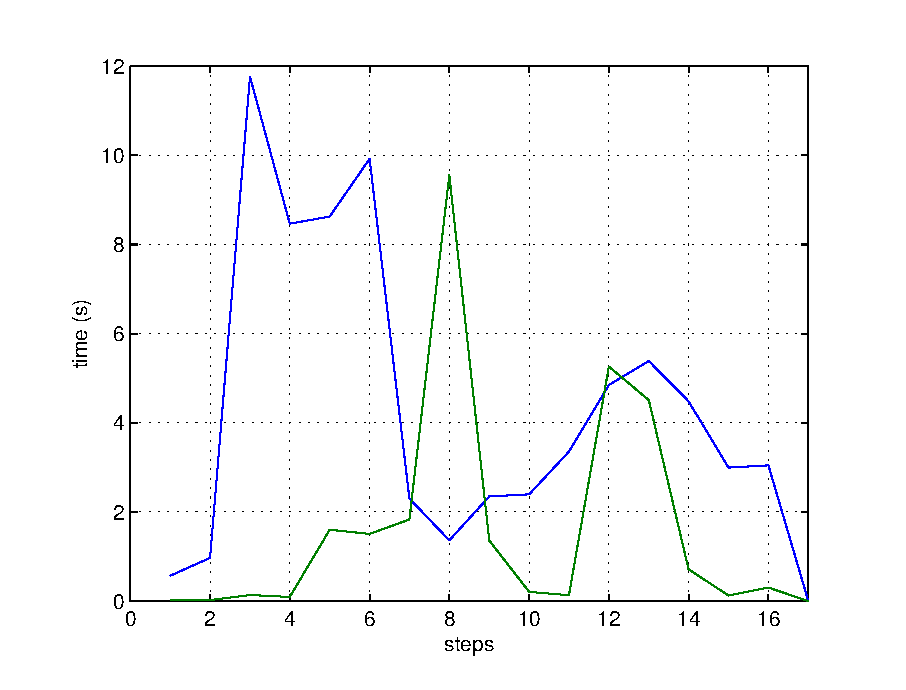
\includegraphics[width=0.48\textwidth]{mini_ab.eps}}
\subfigure[log scale]{
\label{m-1-0} %% label for second subfigure
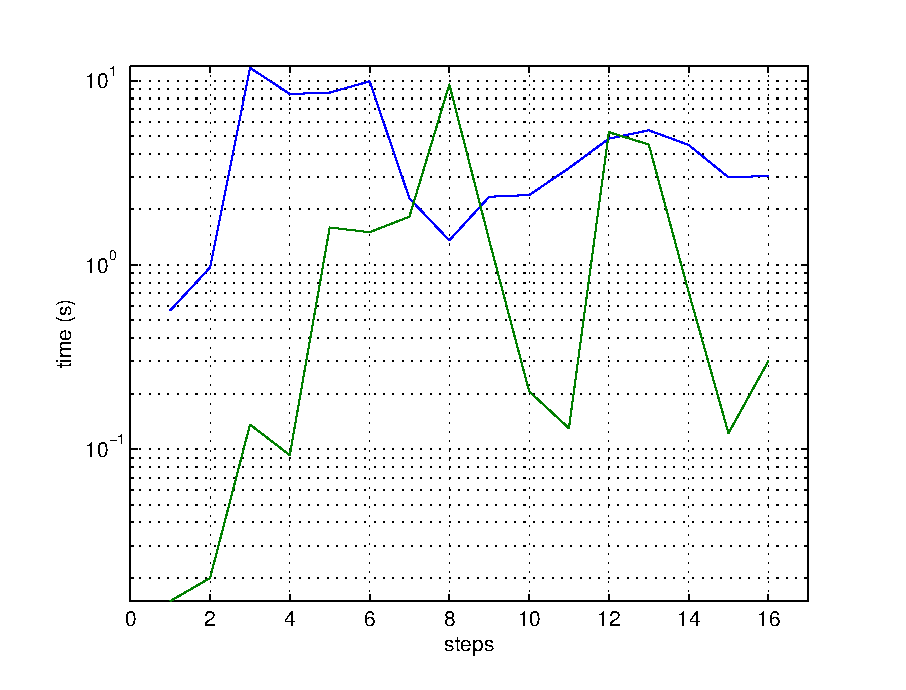
\includegraphics[width=0.48\textwidth]{mini_ab2.eps}}
\caption{step and time curve of Random MinimaxAI and $\alpha\beta$ pruning.}
\label{miniab} %% label for entire figure
\end{figure*}

Figure \ref{abtrans} demonstrate the step and time curve difference when there exists a tranposition table. As expected, the time conusmption is lower when implemented with transposition table. What's more, with transposition table it actually finish the game even fater! Because sometimes the table provider more depth of information than current node, which might lead to a bette decision.

Figure \ref{transorder} demonstrate the step and time curve difference when there exists a tranposition table. Though the time decrease even more significantly, the takes more steps for some unknown reason. I also test ordering enhancement against pure transposition table, it shows that after reodering it becomes a little more stupid. This leave as my future work.

Figure \ref{meantime} demonstrate mean time of different methods. It seems that null-move actually takes more time. I think it becuase although it reduce depth of search occassionally, it actually increase searching times on the same depth. May be I haven't tuned it properly. 

\begin{figure*}[!h]
\centering
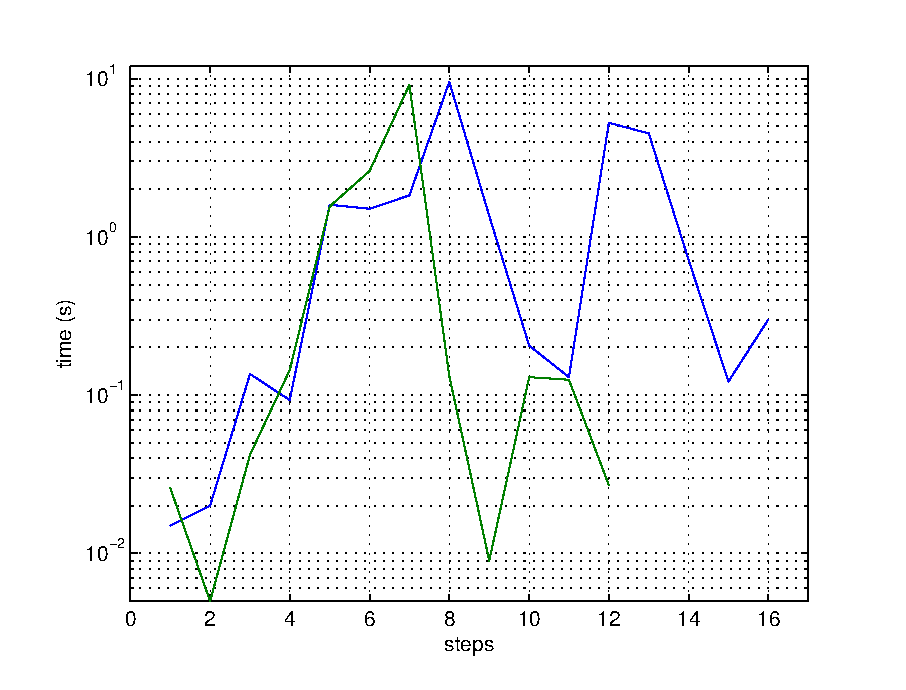
\includegraphics[width=0.48\textwidth]{mini_trans.eps}
\caption{step and time curve of $\alpha\beta$ pruning and$\alpha\beta$ enhanced with transposition table }
\label{abtrans}
\end{figure*}

\begin{figure*}[!h]
\centering
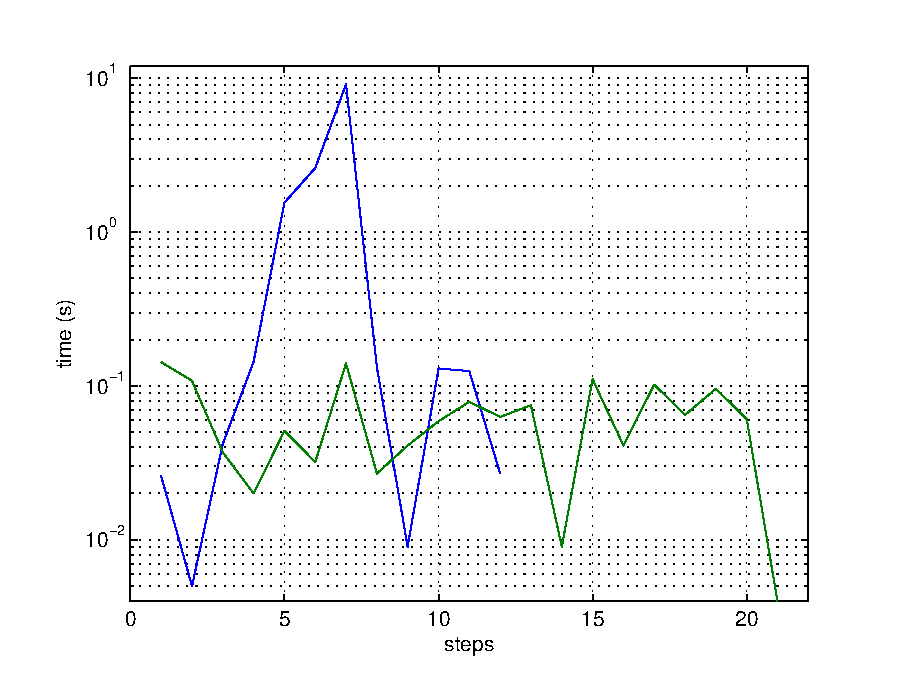
\includegraphics[width=0.48\textwidth]{trans_order.eps}
\caption{step and time curve of transposition table and$\alpha\beta$ enhanced with re-ordering}
\label{transorder}
\end{figure*}

\begin{figure*}[!h]
\centering
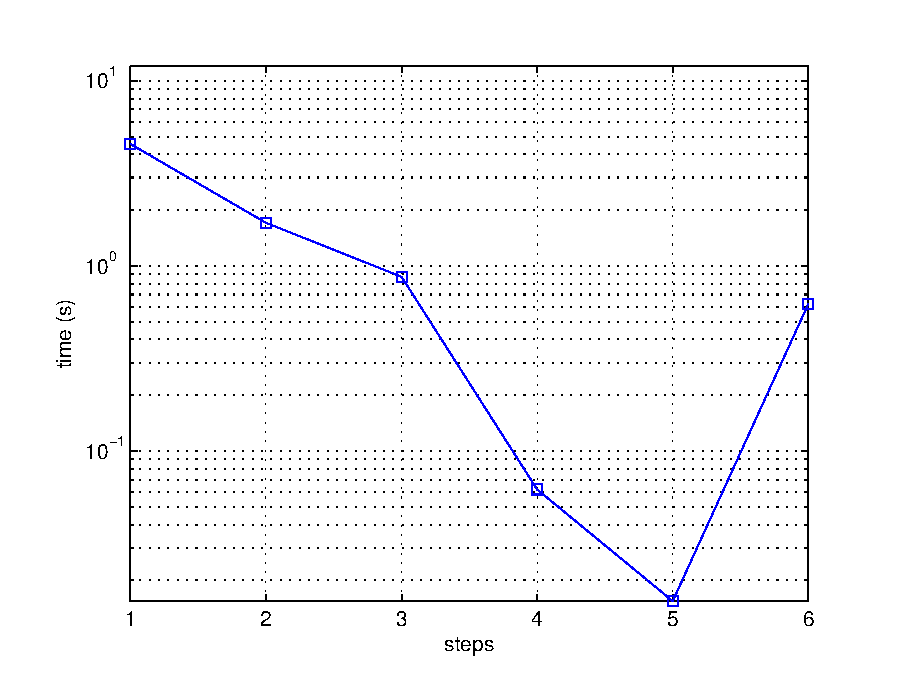
\includegraphics[width=0.48\textwidth]{meantime.eps}
\caption{mean time regards to Minimax, Alpha-beta pruning, transposition table, moves reodering, quiescence search and null move heuristic  repectively}
\label{meantime}
\end{figure*}


\clearpage
\section{Some related work}

Null move strategy can be very tricky. Adaptive Null-Move Pruning \footnote{Heinz, Ernst A. "Adaptive null-move pruning." Scalable Search in Computer Chess. Vieweg+ Teubner Verlag, 2000. 29-40.} prose some good suggestions. 1) when depth is less or equal to 6, use $R=2$. When Depth is larger than 8, use $R=3$. When depth is 6 or 7, and both sides has more than 3 stones, then $R = 3$. Otherwise, R = 2.




\end{document}